\documentclass[]{article}
\usepackage{graphicx}
\usepackage[svgnames]{xcolor} 
\usepackage{fancyhdr}
\usepackage{float}

\usepackage{hyperref}
\usepackage{enumitem}
\usepackage[many]{tcolorbox}
\usepackage{listings }
\usepackage[a4paper, total={6in, 8in}]{geometry}
\usepackage{afterpage}
\usepackage{amssymb}
\usepackage{xepersian}
\usepackage[T1]{fontenc}
\usepackage{tikz}
\usepackage[utf8]{inputenc}
\usepackage{PTSerif} 
\usepackage{seqsplit}

\usepackage{listings}
\usepackage{xcolor}
 
\definecolor{codegreen}{rgb}{0,0.6,0}
\definecolor{codegray}{rgb}{0.5,0.5,0.5}
\definecolor{codepurple}{rgb}{0.58,0,0.82}
\definecolor{backcolour}{rgb}{0.95,0.95,0.92}
 
\NewDocumentCommand{\codeword}{v}{
\texttt{\textcolor{blue}{#1}}
}
\lstset{language=C,keywordstyle={\bfseries \color{blue}}}

\lstdefinestyle{mystyle}{
    backgroundcolor=\color{backcolour},   
    commentstyle=\color{codegreen},
    keywordstyle=\color{magenta},
    numberstyle=\tiny\color{codegray},
    stringstyle=\color{codepurple},
    basicstyle=\ttfamily\normalsize,
    breakatwhitespace=false,         
    breaklines=true,                 
    captionpos=b,                    
    keepspaces=true,                 
    numbers=left,                    
    numbersep=5pt,                  
    showspaces=false,                
    showstringspaces=false,
    showtabs=false,                  
    tabsize=2
}
\lstset{style=mystyle}

\settextfont[BoldFont={XB Zar bold.ttf}]{XB Zar.ttf}




\newcommand{\inputsample}[1]{
    ~\\
    \textbf{ورودی نمونه}
    ~\\
    \begin{tcolorbox}[breakable,boxrule=0pt]
        \begin{latin}
            \large{
                #1
            }
        \end{latin}
    \end{tcolorbox}
}
\newcommand\tab[1][1cm]{\hspace*{#1}}
\newcommand{\outputsample}[1]{
    ~\\
    \textbf{خروجی نمونه}

    \begin{tcolorbox}[breakable,boxrule=0pt]
        \begin{latin}
            \large{
                #1
            }
        \end{latin}
    \end{tcolorbox}
}

%%%%%باکس های طراحی شده برای پاسخ نامه ، میتوانید پاسخ را درون باکس قراردهید
\newtcolorbox[auto counter]{solutionbox}{
freelance,
colback=white,
frame code={},
interior titled code={
  \fill[rounded corners=8pt,orange!30]
    (title.south west) --
    (title.south) -- 
    ([yshift=20pt]title.south) --
    ([yshift=20pt,xshift=4cm]title.south) --
    ([xshift=4cm]title.south) --
    (title.south east) {[sharp corners] --
    ([yshift=-6pt]title.south east) -- 
    ([yshift=-6pt]title.south west) } -- cycle;
  \draw[rounded corners=8pt,gray,line width=1pt]
    (title.west|-frame.south west) --
    (title.south west) --
    (title.south) -- 
    ([yshift=20pt]title.south) --
    ([yshift=20pt,xshift=4cm]title.south) --
    ([xshift=4cm]title.south) --
    (title.south east) --
    (title.east|-frame.south east) --
    cycle;
  \node at ([xshift=2cm,yshift=4pt,anchor=south]title.south) 
    {\Large \textbf{پاسخ}};  
  },
title={\mbox{}},
top=12pt,
fontupper=\sffamily\Large,
oversize=0.5cm,
before={\vskip24pt\par\noindent},
after={\par\vskip12pt}
}
\newtcolorbox[auto counter]{solutionboxC}{
freelance,
colback=white,
frame code={},
interior titled code={
  \fill[rounded corners=8pt,orange!30]
    (title.south west) --
    (title.south) -- 
    ([yshift=20pt]title.south) --
    ([yshift=20pt,xshift=4cm]title.south) --
    ([xshift=4cm]title.south) --
    (title.south east) {[sharp corners] --
    ([yshift=-6pt]title.south east) -- 
    ([yshift=-6pt]title.south west) } -- cycle;
  \draw[rounded corners=8pt,gray,line width=1pt]
    (title.west|-frame.south west) --
    (title.south west) --
    (title.south) -- 
    ([yshift=20pt]title.south) --
    ([yshift=20pt,xshift=4cm]title.south) --
    ([xshift=4cm]title.south) --
    (title.south east) --
    (title.east|-frame.south east) --
    cycle;
  \node at ([xshift=2cm,yshift=4pt,anchor=south]title.south) 
    {\Large \textbf{ پاسخ ادامه}};  
  },
title={\mbox{}},
top=12pt,
fontupper=\sffamily\Large,
oversize=0.5cm,
before={\vskip24pt\par\noindent},
after={\par\vskip12pt}
}

\begin{document}


%%% title pages
\begin{titlepage}
\begin{center}
        
\vspace*{0.7cm}


\includegraphics[width=0.4\textwidth]{sharif1.png}\\
\vspace{0.5cm}
\textbf{ \Huge{\emph درس برنامه‌سازی پیشرفته} }\\
\vspace{0.5cm}
\textbf{ \Large{ تمرین سوم بخش دوم} }
\vspace{0.2cm}
       
 
      \large \textbf{دانشکده مهندسی کامپیوتر}\\\vspace{0.2cm}
    \large   دانشگاه صنعتی شریف\\\vspace{0.2cm}
       \large   ﻧﯿﻢ سال دوم 99-98 \\\vspace{0.2cm}
      \noindent\rule[1ex]{\linewidth}{1pt}
    مبحث:\\
    \textbf{{همروندی}}

    \vspace{0.20cm}

   مهلت ارسال:\\
    \textbf{{5 دی}}\\
    \textbf{{ساعت 23:59}}

    \vspace{0.15cm}
ویراستار فنی:\\
    \textbf{{محمدمهدی ابوترابی و پارسا محمدیان}}
\end{center}
\end{titlepage}
%%% title pages


%%% header of pages
\newpage
\pagestyle{fancy}
\fancyhf{}
\fancyfoot{}
\cfoot{\thepage}
\chead{همروندی}
\rhead{
\includegraphics[width=0.1\textwidth]{sharif.png}}
\lhead{تمرین 2.3 برنامه‌سازی پیشرفته}
%%% header of pages




 \Large \textbf{\\\\
به موارد زیر توجه کنید:}

\begin{itemize}[label=$\ast$]
\item  فایل برنامه‌ی خود با پسوند .zip را در بخش مربوط به سوال بارگذاری کنید. 
کد شما موقع تحویل حضوری بررسی و نمره‌دهی می‌شود.
\item هم‌فکری و هم‌کاری در پاسخ به تمرینات اشکالی ندارد و حتی توصیه نیز می‌شود؛ ولی پاسخ ارسالی شما باید حتما توسط خود شما نوشته شده‌باشد. در صورت هم‌فکری در مورد یک سوال، نام افراد دیگر را به‌صورت کامنت در ابتدای کد هر سوال بنویسید.  این نکته رو در نظر بگیرید که هم‌فکری تنها مربوط به بخش ایده سوال هست نه پیاده‌سازی آن و در صورت محرز شدن تقلب برای فرد خاطی بدون مسامحه \emph{ منفی نمره تمرین}
منظور می‌گردد. 
\item شما می‌توانید تمامی سوالات و ابهامات خود را در سایت کوئرا در بخش مشخص‌شده برای این تمرین بپرسید.
\item به‌ازای هر روز تاخیر در ارسال پاسخ هر سوال، 30 درصد از نمره‌ی کسب‌شده‌ی شما در آن سوال کم می‌شود. به عنوان مثال اگر پاسخ یک سوال را با دو روز تاخیر ارسال کنید، فقط 40 درصد از نمره‌ای که برای آن سوال گرفته‌اید برای شما لحاظ خواهد شد.
\item در کل شما می‌توانید سه روز تاخیر بدون کسر نمره داشته باشد.
\item مهلت ارسال تمرین تا ساعت 23:59 روز 5 دی 1399 است.
\end{itemize}



\newpage

\section{شبیه‌سازی سیستم کنترل هوشمند ترافیک(50 نمره)}
دو چهارراه 1 و 2 را در نظر بگیرید که همه‌ی خیابان‌های مرتبط با آن‌ها یک‌طرفه (چپ 
به راست یا بالا به پایین) است و دور زدن و گردش به چپ و راست در آن‌ها ممنوع 
است 
(خودروها فقط مستقیم حرکت می‌کنند). یک مشکل اساسی داریم که فضای بین دو 
چهارراه 
فقط به اندازه‌ی n خودرو ظرفیت دارد. بر سر راه خودروهایی که از چپ به راست حرکت 
می‌کنند، دو چراغ راهنما یکی در چهارراه 1 و دیگری در چهارراه 2 تعبیه شده است. 
در حالت معمول، چراغ راهنمای 1 و 2 هر کدام به شکل مستقل به اندازه‌ی 1، 2 یا 3 
ثانیه (احتمال هر یک از این سه برابر است و به شکل تصادفی انتخاب می‌شود) قرمز 
هستند و سپس به اندازه‌ی عبور فقط یک ماشین سبز می‌شوند (از نظر زمانی ناچیز است) 
و این روند تا بی‌نهایت ادامه دارد. با توجه به محدود بودن ظرفیت بین دو چهارراه  
(n)، استثنائی در سبز و قرمز شدن چراغ‌ها اعمال شده است و آن این است که اگر 
فضای بین دو چهارراه پر باشد، چراغ 1 در حالت قرمز منتظر می‌ماند تا چراغ 2 به 
او خبر دهد که حداقل یک فضای خالی ایجاد شده است (بدیهی است که چراغ 2 پس از 
سبز شدن این خبر را ارسال می‌کند). یک استثناء دیگر آن است که به منظور کاهش 
میزان انتظار خودروها، اگر هیچ خودرویی بین دو چهارراه نباشد، چراغ 2 در حالت 
قرمز منتظر می‌ماند تا چراغ 1 به او خبر دهد که حداقل یک خودرو وارد فضای بین دو 
چهارراه شده است. مطلوبست نوشتن برنامه‌ی کاملی که این سیستم را شبیه‌سازی نماید. 
برنامه تا ابد ادامه می‌یابد و خروجی آن تمام رخدادهایی است که در سیستم رخ 
می‌دهد (به ازای هر یک از دو چراغ راهنما یک نخ مجزا و به ازای خیابان بین دو 
چهارراه یک لیست به ظرفیت n در نظر بگیرید. n در ابتدای کار از کاربر پرسیده 
می‌شود). فرض بر این است که پشت چراغ قرمز اول همواره ماشین وجود دارد و پس از 
سبز شدن آن یک ماشین وارد خیابان بین دو چهارراه می شود. برای طی مسافت خیابان 
بین دو چهارراه توسط ماشین لازم نیست زمانی در نظر بگیرید.

\begin{figure}[H]
	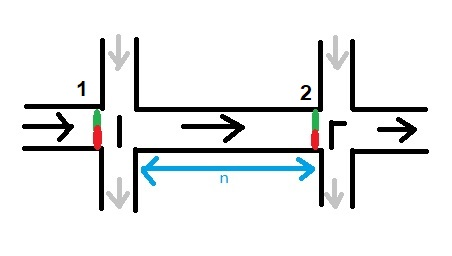
\includegraphics[width=\linewidth]{example.png}
	\caption{مثال}
	\label{}
\end{figure}

\begin{itemize}
\item
در ابتدا باید ورودی n را از کاربر بگیرید. ابتدا پیام زیر را چاپ کنید. برای 
این کار اگر کاربر مقدار غیر معتبری وارد کرد باید این قدر برنامه شما منتظر 
بماند تا کاربر عدد مناسب وارد کند.(در واقع با ورودی غیر معتبر برنامه شما 
پایان نیابد)(n حداقل یک است و میتوان آن را integer در نظر بگیرید.)
\begin{tcolorbox}[boxrule=0pt]
	\begin{latin}
		\large{
			Enter capacity:
		}
	\end{latin}
\end{tcolorbox}

\item
در صورت نا معتبر بودن ورودی پیام زیر را بدهید.
\begin{tcolorbox}[boxrule=0pt]
	\begin{latin}
		\large{
			Not valid format
		}
	\end{latin}
\end{tcolorbox}

\item
هر چراغ که خواست به خواب برود و قرمز بماند باید پیام زیر را چاپ کند.(m 
تعداد ثانیه که همان عدد رندم است و k هم شماره چراغ است که 1 یا 2 است.)
\begin{tcolorbox}[boxrule=0pt]
	\begin{latin}
		\large{
			Traffic light k is red for m second
		}
	\end{latin}
\end{tcolorbox}

\item
اگر فضای بین دو چراغ از ماشین پر شده بود و چراغ اول مجبور بود کماکان قرمز 
باقی بماند پیام زیر چاپ می‌شود.
\begin{tcolorbox}[boxrule=0pt]
	\begin{latin}
		\large{
			Traffic light 1 is still red and waits for traffic light 2 to 
			reduce number of cars
		}
	\end{latin}
\end{tcolorbox}

\item
اگر چراغ دوم مجبور بود کماکان قرمز بماند پیام زیر چاپ شود.
\begin{tcolorbox}[boxrule=0pt]
	\begin{latin}
		\large{
			Traffic light 2 is still red and waits for traffic light 1 to add a 
			car into it
		}
	\end{latin}
\end{tcolorbox}

\item
وقتی چراغ اول سبز می‌شود و یک ماشین از چراغ رد می‌شود پیام های زیر چاپ شود.
\begin{tcolorbox}[boxrule=0pt]
	\begin{latin}
		\large{
			Traffic light 1 is green and 1 car moved from traffic light 1 to 
			traffic light 2
		}
	\end{latin}
\end{tcolorbox}
(\lr{X}همان تعداد ماشین های پشت چراغ دوم است.)
\begin{tcolorbox}[boxrule=0pt]
	\begin{latin}
		\large{
			Now there are X cars behind traffic light 2
		}
	\end{latin}
\end{tcolorbox}

\item
اگر چراغ دوم سبز شد و ماشینی از آن عبور کرد پیام زیر چاپ شود.
\begin{tcolorbox}[boxrule=0pt]
	\begin{latin}
		\large{
			Traffic light 2 is green and a car removed from traffic light 2 and 
			now there are X cars behind traffic light 2
		}
	\end{latin}
\end{tcolorbox}
\end{itemize}

\newpage

\section{بخش امتیازی(20 نمره)}
در این بخش باید رابطی گرافیکی برای شبیه‌سازی سیستم کنترل هوشمند ترافیک (کدی 
که در قسمت قبل زدید) طراحی کنید. دستتان برای طراحی رابط گرافیکی باز است. 
رابط کاربری گرافیکی شما موقع تحویل حضوری بررسی خواهد شد. پیشنهاد می‌شود برای 
انجام این قسمت کد قسمت قبلی خود را با رعایت اصول تمیزی کد بنویسید. 

\end{document}
